\section{Aplikace ve výuce a didaktický přínos}

\subsection{Výukový cíl}
Primárním cílem této pomůcky je pomoci studentům a učitelům přehledně rozdělit daná témata v určitém období a přidat k nim potřebný kontext, případně srovnání s jinými událostmi. K jednotlivým událostem také patří jejich popis a další informace, které jsou vhodné i pro učení látky jako takové.

\subsection{Didaktické zařazení}
Tato aplikace nabízí možnost využití napříč různými odvětvími. Mezi hlavní patří dějepis, literatura, hudební či výtvarné umění v rámci historie. V těchto předmětech by Tempora mohla být použita jako jedna z hlavních výukových pomůcek. Své uplatnění by ale mohla najít i mimo humanitní vědy, a to ve více technických předmětech, jako je fyzika, chemie, biologie a další, kde by pomohla přiblížit historický kontext objevů a důležitých vynálezů. Zde by mohla sloužit pouze jako vedlejší pomůcka studentům k srovnání jednotlivých letopočtů a dat daných událostí. Tato aplikace je vhodná pro použití od druhého stupně základní školy až do vyšších ročníků středních škol a gymnázií.



\subsection{Využití ve výuce}
Využití v samotných hodinách může mít různou formu. Učitel si může připravit osu na dané téma a ukazovat na ní jednotlivá období. Odkaz na tuto osu pak může pomocí například Google Classroom nebo Microsoft Teams nasdílet do učebny pro samostatné studium. Další možností je zadat nějaké téma a nechat ho zpracovat studenty v hodině, následně jej prezentovat před třídou. Učitel může také zadat tvorbu osy jako dobrovolný či povinný domácí úkol.



\subsection{Dotazník pro studenty}
\label{Dotazník}

Abych zjistil, co si o aplikaci myslí studenti, nechal jsem otestovat svůj projekt několika spolužáky, kteří mi následně vyplnili dotazník. Ten bych zde chtěl rozebrat.

\subsubsection{Testování aplikace}
Aplikaci jsem nasadil na vlastní server a pomocí služby Ngrok\cite{ngrok} sdílel vygenerovanou zabezpečenou URL. Tento způsob jsem zvolil pouze pro testování a v rámci rychlého sdílení projektu. Pokud by se projekt měl aplikovat ve velkém měřítku, je samozřejmě možné pomocí Dockeru aplikaci nasadit na placený server s vlastní doménou.


\subsubsection{Výsledky průzkumu}
V dotazníku vytvořeném v Google Forms jsem se ptal na různé aspekty aplikace – od zkušeností s používáním, přes nalezené problémy až po její využití ve výuce.
Pro mě nejdůležitějším tématem byla přehlednost a jednoduchost aplikace, na což jsem se zeptal v otázkách 1 a 2 (obrázek \ref{fig:graf12}).

\begin{figure}[h]
\begin{minipage}[]{0.5\linewidth}
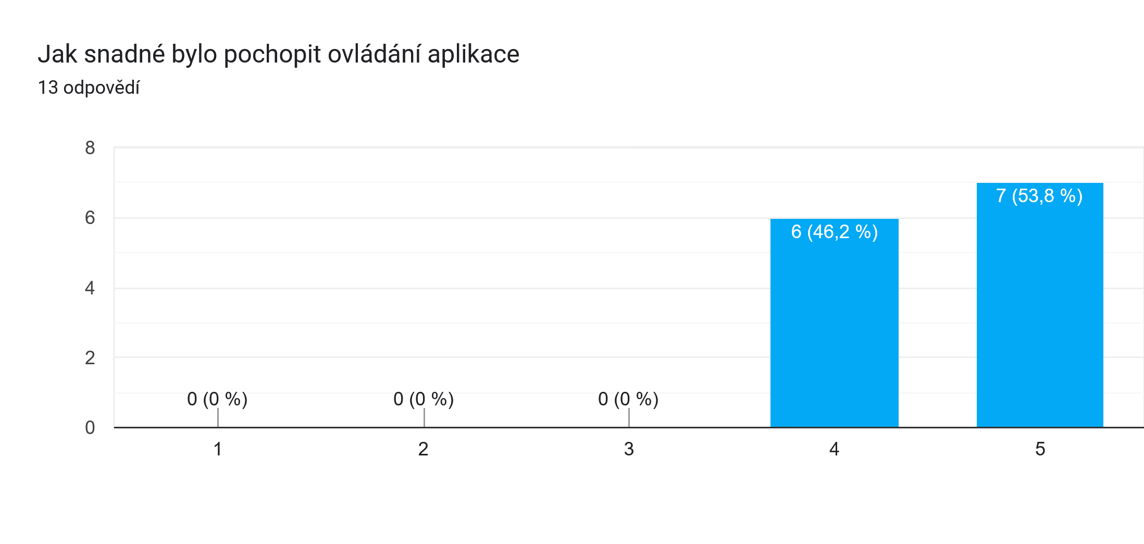
\includegraphics[width=\linewidth]{Images/graf1.png}
\end{minipage}
\hfill
\begin{minipage}[]{0.5\linewidth}
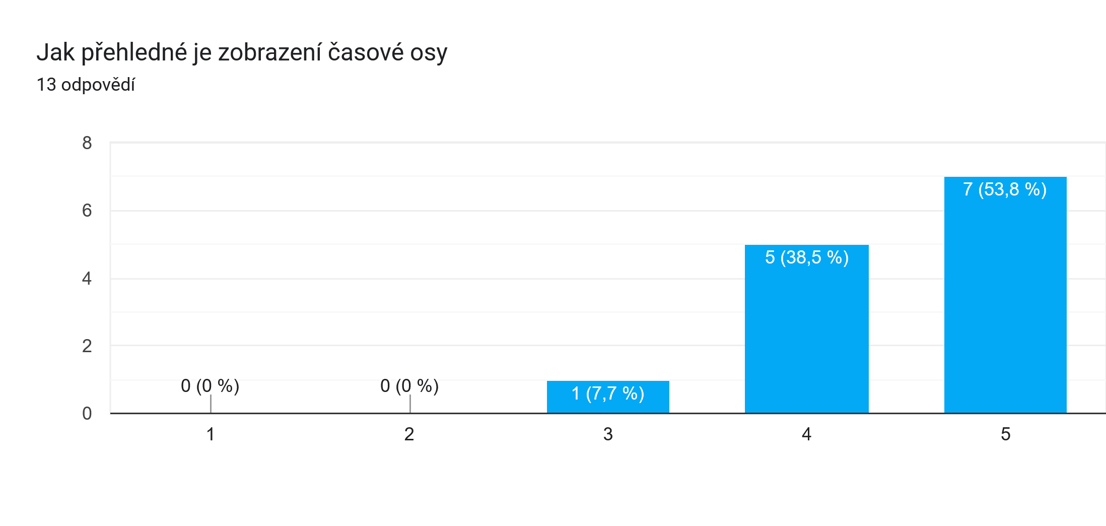
\includegraphics[width=\linewidth]{Images/graf2.png}
\end{minipage}%
\caption{Grafy první a druhé otázky dotazníku}
\label{fig:graf12}
\end{figure}

Z grafu jednoznačně vyplývá, že můj záměr byl úspěšný – respondenti označili aplikaci jako velmi snadnou a přehlednou. Stejný závěr měla i otázka 3: Jak užitečné jsou vizuální prvky (barvy, rozložení, styl), kde byly nejčastěji zvoleny možnosti 4 nebo 5 (5 = velmi užitečné).

\begin{figure}[h]
    \centering
    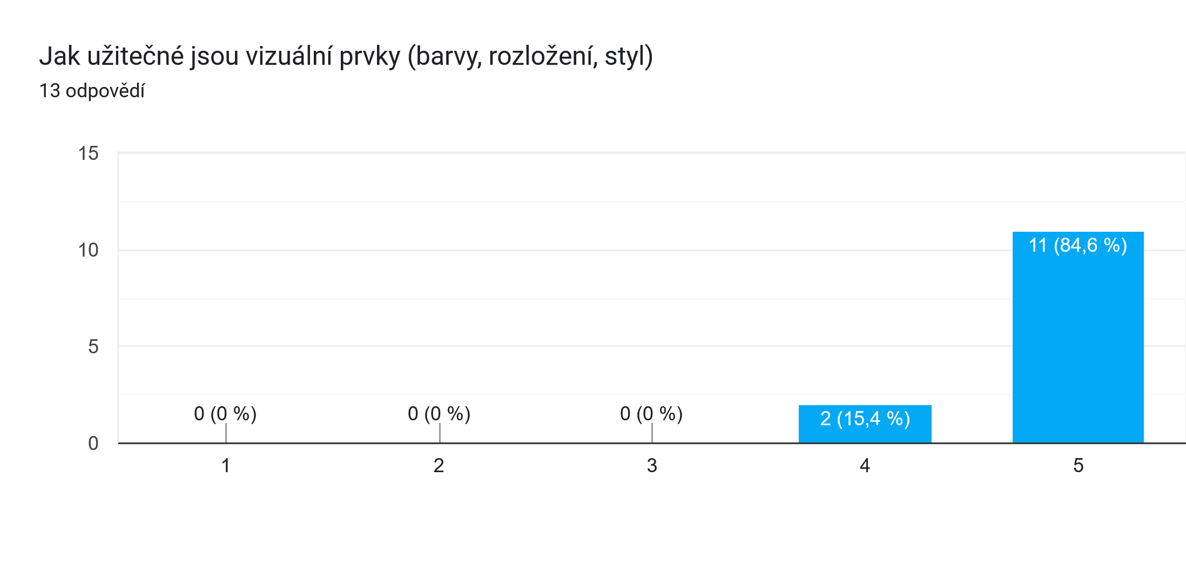
\includegraphics[width=0.8\linewidth]{Images/graf3.png}
    \caption{Graf 3. otázky dotazníku}
    \label{fig:graf3}
\end{figure}

\newpage
Čtvrtá otázka se věnovala využití aplikace ve výuce s historickým kontextem. S velkou převahou vede odpověď: Používal bych tuto aplikaci v kombinaci s jinými zdroji, což znamená, že aplikace je užitečná, ale nenahrazuje kompletně ostatní výukové prostředky.

\begin{figure}[h]
    \centering
    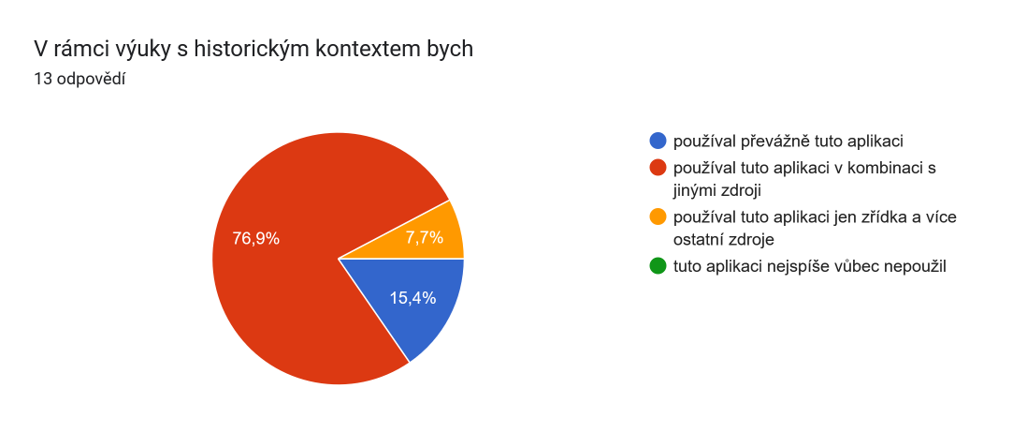
\includegraphics[width=0.8\linewidth]{Images/graf4.png}
    \caption{Graf 4. otázky dotazníku}
    \label{fig:graf4}
\end{figure}

V otázce číslo pět jsem se respondentů zeptal, jak si představují využití aplikace ve výuce. Tato otázka umožňovala více vybraných možností (viz obrázek \ref{fig:graf5}).

\begin{figure}[h]
    \centering
    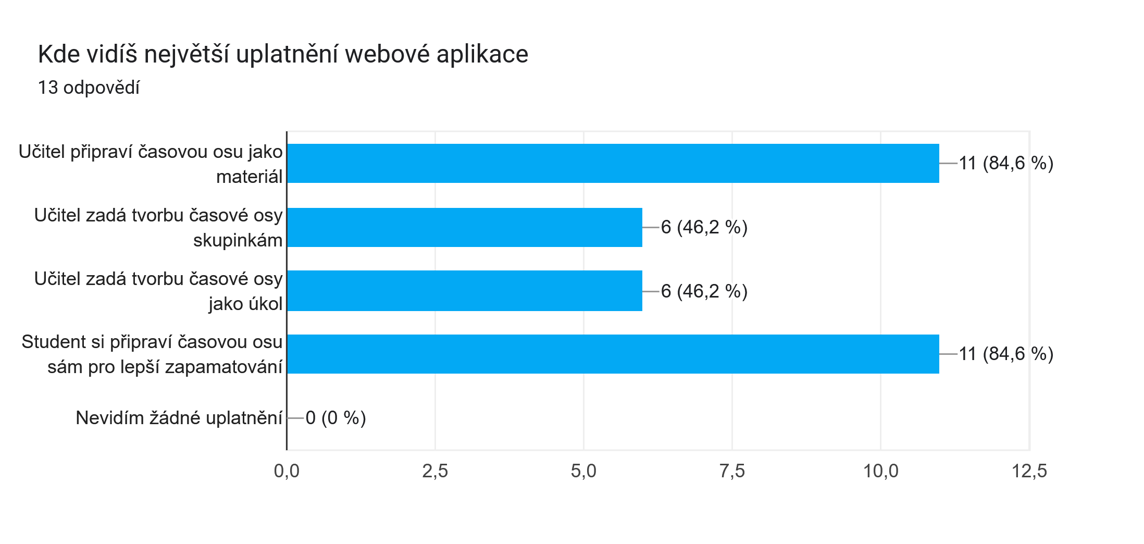
\includegraphics[width=0.8\linewidth]{Images/graf5.png}
    \caption{Graf 5. otázky dotazníku}
    \label{fig:graf5}
\end{figure}


Na prvním místě se shodným počtem hlasů umístily odpovědi 1 a 4.
O zhruba polovinu hlasů méně získaly odpovědi 2 a 3.
Tento výsledek ukazuje, že studenti více preferují použití osy samostatně před skupinovou prací a dávají přednost studiu z vlastní iniciativy nebo výuce z učitelovy časové osy před povinným úkolem.

V poslední části dotazníku jsem se ptal na zpětnou vazbu a možná vylepšení, která respondenty napadla.

Jedna z odpovědí si stěžovala na zpočátku těžce pochopitelné ovládání.
Tento problém by se dal vyřešit přidáním stránky s návodem nebo navedením nového uživatele pomocí vysvětlivek, jak časová osa funguje.
Další dotaz se týkal možnosti zadání přesného data. Tato funkce nebyla přidána kvůli zjednodušení databázového systému a proto, že osa má sloužit primárně k zobrazování delších období. Pokud však uživatel chce zdůraznit určité datum, může jej uvést do názvu období.